\documentclass[12pt,a4paper]{article}
\usepackage{graphicx}
\usepackage{amssymb}

% put your student ID here instead of 1234567

\newcommand{\thestudentid}{2546379}

% put the number of the question you are answering here, instead of 0

\newcommand{\theexam}{Data Structures, Algorithms \& Databases}

\author{ID \thestudentid}
\title{Exam for \theexam}
\date{}

\usepackage{cmbright}
\usepackage{fullpage}
\usepackage{fancyhdr}

\pagestyle{fancyplain}
\setlength{\headheight}{15pt}
\lhead{\fancyplain{ID \thestudentid}{ID \thestudentid}}
\rhead{\fancyplain{Exam for \theexam}{\theexam}}
\lfoot{\fancyplain{ID \thestudentid}{ID \thestudentid}}
\rfoot{\fancyplain{\theexam}{\theexam}}

\usepackage{hyperref}
\newcounter{question}\setcounter{question}{1}
\newenvironment{question}{%
\subsection*{Question \arabic{question}}}%
{\stepcounter{question}}

\begin{document}


\maketitle


\begin{question}
Part 1
\begin{table}[h]
\centering
\begin{tabular}{|c|c|}
\hline
N[v] & Neighbours(s) \\
\hline
A & (B, 7), (C, 4), (E, 8) \\
\hline
B & (A, 7), (C, 3), (E, 2) \\
\hline
C & (A, 4), (B, 3), (D, 9) \\
\hline
D & (C, 9), (E, 6), (F, 7) \\
\hline
E & (A, 8), (B, 2), (D, 6), (F, 7) \\
\hline
F & (D, 7), (E, 5) \\
\hline
\end{tabular}
\caption{Part 1}
\label{tab:1}
\end{table}

Part 2
\begin{figure}[h]
  \centering
  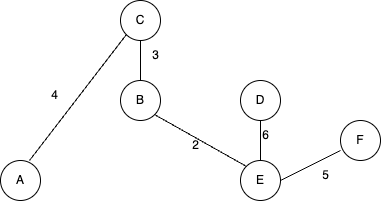
\includegraphics[width=0.5\textwidth]{part2.png}
  \caption{Total Weight: 20}
  \label{fig:my_graph}
\end{figure}
\end{question}
\newpage

\begin{question}
\begin{table}[h]
\centering
\begin{tabular}{|c|c|c|c|c|c|}
\hline
A & B & C & D & E & Finished \\
\hline
0, A & $\infty$, B & $\infty$, C & $\infty$, D & $\infty$, E & \\
\hline
0, A, $\checkmark$ & 5, A & $\infty$, C & 13, A & 20, A & A \\
\hline
0, A, $\checkmark$ & 5, A, $\checkmark$ & 8, B & 13, A & 17, B & B\\
\hline
0, A, $\checkmark$ & 5, A, $\checkmark$ & 8, B $\checkmark$ & 10, C & 17, B & C \\
\hline
0, A, $\checkmark$ & 5, A, $\checkmark$ & 8, B $\checkmark$ & 10, C $\checkmark$ & 13, D & D \\
\hline
0, A, $\checkmark$ & 5, A, $\checkmark$ & 8, B $\checkmark$ & 10, C $\checkmark$ & 13, D $\checkmark$ & E \\
\hline
\end{tabular}
\caption{}
Total Weight: 13 \\
Shortest Path: $A \rightarrow B \rightarrow C \rightarrow D \rightarrow E$ \\
\label{tab:2}
\end{table}
\end{question}


\begin{question}
\raggedright
\begin{itemize}
\item linear probing \\
    \begin{enumerate}
        \item
        		\begin{tabular}{|c|c|c|c|c|c|}
       	 	\hline
       		 0 & 1 & 2 & 3 & 4 & 5 \\
       		 \hline
       		 & B & D & E & A & \\
        		\hline
        		\end{tabular}
        \item
        		\begin{tabular}{|c|c|c|c|c|c|}
       	 	\hline
       		 0 & 1 & 2 & 3 & 4 & 5 \\
       		 \hline
       		 & B & D & E & A & C \\
        		\hline
        		\end{tabular}
        \item
        		\begin{tabular}{|c|c|c|c|c|c|}
       	 	\hline
       		 0 & 1 & 2 & 3 & 4 & 5 \\
       		 \hline
       		 F & B & D & E & A & C \\
        		\hline
        		\end{tabular}
        \item
        		\begin{tabular}{|c|c|c|c|c|c|}
       	 	\hline
       		 0 & 1 & 2 & 3 & 4 & 5 \\
       		 \hline
       		 F & B & \# & E & A & C \\
        		\hline
        		\end{tabular}
        \item
        		\begin{tabular}{|c|c|c|c|c|c|}
       	 	\hline
       		 0 & 1 & 2 & 3 & 4 & 5 \\
       		 \hline
       		 F & B & \# & E & A & \# \\
        		\hline
        		\end{tabular}
        \item
        		\begin{tabular}{|c|c|c|c|c|c|}
       	 	\hline
       		 0 & 1 & 2 & 3 & 4 & 5 \\
       		 \hline
       		 F & B & C & E & A & \# \\
        		\hline
        		\end{tabular}
    \end{enumerate}
\newpage
\item double hashing \\
    \begin{enumerate}
        \item
        		\begin{tabular}{|c|c|c|c|c|c|}
       	 	\hline
       		 0 & 1 & 2 & 3 & 4 & 5 \\
       		 \hline
       		 & B & D & E & \# & A\\
        		\hline
        		\end{tabular}
        \item
        		\begin{tabular}{|c|c|c|c|c|c|}
       	 	\hline
       		 0 & 1 & 2 & 3 & 4 & 5 \\
       		 \hline
       		 & B & D & E & C & A \\
        		\hline
        		\end{tabular}
        \item
        		\begin{tabular}{|c|c|c|c|c|c|}
       	 	\hline
       		 0 & 1 & 2 & 3 & 4 & 5 \\
       		 \hline
       		 F & B & D & E & C & A \\
        		\hline
        		\end{tabular}
        \item
        		\begin{tabular}{|c|c|c|c|c|c|}
       	 	\hline
       		 0 & 1 & 2 & 3 & 4 & 5 \\
       		 \hline
       		 F & B & \# & E & C & A \\
        		\hline
        		\end{tabular}
        \item
        		\begin{tabular}{|c|c|c|c|c|c|}
       	 	\hline
       		 0 & 1 & 2 & 3 & 4 & 5 \\
       		 \hline
       		 F & B & \# & E & \# & A \\
        		\hline
        		\end{tabular}
        \item
        		\begin{tabular}{|c|c|c|c|c|c|}
       	 	\hline
       		 0 & 1 & 2 & 3 & 4 & 5 \\
       		 \hline
       		 F & B & C & E & \# & A \\
        		\hline
        		\end{tabular}
    \end{enumerate}
\end{itemize}
\end{question}


 \vspace*{1cm}
\pagebreak[3]\fbox{%
\begin{minipage}[c]{0.92\textwidth}
\raggedright
Statement of good academic conduct

By submitting this assignment, I understand that I am agreeing to the
following statement of good academic conduct.
\begin{itemize}
\item
I confirm that this assignment is my own work and I have not worked
with others in preparing this assignment.
\item
I confirm this assignment was written by me and is in my own words,
except for any materials from published or other sources which are
clearly indicated and acknowledged as such by appropriate referencing.
\item
I confirm that this work is not copied from any other person's work
(published or unpublished), web site, book or other source, and has
not previously been submitted for assessment either at the University
of Birmingham or elsewhere.
\item
I confirm that I have not asked, or paid, others to prepare any part
of this work for me.
\item
I confirm that I have read and understood the
\href{https://intranet.birmingham.ac.uk/as/registry/policy/conduct/plagiarism/index.aspx}{University
  regulations on plagiarism}.
\end{itemize}

\end{minipage}%
}
\end{document}
